%%%%%%%%%%%%%%%%%%%%%%%%%%%%%%%%%%%%%%%%%%%%%%%%%%%%%%%%%%%%%%%%%%%%%%%%%%%%%%%%
%2345678901234567890123456789012345678901234567890123456789012345678901234567890
%        1         2         3         4         5         6         7         8

\documentclass[letterpaper, 10 pt, conference]{ieee/ieeeconf}  % Comment this line out if you need a4paper

%\documentclass[a4paper, 10pt, conference]{ieeeconf}      % Use this line for a4 paper

\IEEEoverridecommandlockouts                              % This command is only needed if 
                                                          % you want to use the \thanks command

\overrideIEEEmargins                                      % Needed to meet printer requirements.

% See the \addtolength command later in the file to balance the column lengths
% on the last page of the document

% The following packages can be found on http:\\www.ctan.org
%\usepackage{graphics} % for pdf, bitmapped graphics files
\usepackage{graphicx} % for jpg
%\usepackage{epsfig} % for postscript graphics files
%\usepackage{mathptmx} % assumes new font selection scheme installed
%\usepackage{times} % assumes new font selection scheme installed
%\usepackage{amsmath} % assumes amsmath package installed
%\usepackage{amssymb}  % assumes amsmath package installed

\usepackage[hidelinks]{hyperref}
\usepackage{todonotes}
\setlength{\marginparwidth}{1.5cm} % For TODOs.
%\usepackage[T1]{fontenc} % For less than signs?
\usepackage{subcaption}
\usepackage{dblfloatfix}
% For lovely checkmarks.
\usepackage{pifont}% http://ctan.org/pkg/pifont
\newcommand{\cmark}{\ding{51}}%
\newcommand{\xmark}{\ding{55}}%
% For footnotes in table.
\usepackage{threeparttable}

%%%%%%%%%%%%%%%%%%%%%%%%%%%%%%%%%%%%%%%%%%%%%%%%%%%%%%%%%%%%%%%%%%%%%%%%%%%%%%%%
\title{\LARGE \bf
A lightweight, cross-platform, multiuser robot visualization \\ using the cloud*
}

\author{William Hilton$^{1}$, Paul Oh$^{2}$, Youngmoo Kim$^{3}$, Dan Lofaro$^{4}$% <-this % stops a space
\thanks{*This work was supported in part by NSF CNS-0960061: MRI-R2 Unifying Humanoids Research.}% <-this % stops a space
\thanks{$^{1}$William Hilton is with Department of Electrical Engineering, Drexel University,
        Philadelphia, PA 19104, USA
        {\tt\small wmhilton@drexel.edu}}%
\thanks{$^{2}$Paul Oh is with Faculty of Mechanical Engineering, Drexel University,
        Philadelphia, PA 19104, USA
        {\tt\small paul@coe.drexel.edu}}%        
\thanks{$^{3}$Youngmoo Kim is with Faculty of Electrical Engineering, Drexel University,
        Philadelphia, PA 19104, USA
        {\tt\small ykim@drexel.edu}}%
\thanks{$^{4}$Dan Lofaro is with Department of Electrical Engineering, George Mason University,
        Fairfax, VA 22030, USA
        {\tt\small dlofaro@gmu.edu}}%
}

\begin{document}
\maketitle
\thispagestyle{empty}
\pagestyle{empty}

%%%%%%%%%%%%%%%%%%%%%%%%%%%%%%%%%%%%%%%%%%%%%%%%%%%%%%%%%%%%%%%%%%%%%%%%%%%%%%%%

% % Youngmoo kim's thoughts
% Education
% Agree to strip DRC out of it
% Strike first figure. Use detailed figure.
% Talk more about pros/cons of Firebase as a database for robot telemetry data
% Latency, race conditions? Real-time telemetry

% Explain the database aspect for Firebase more. Stores data. Triggers updates.

% Give some more example applications
% Roboticist wants an interface that's fast and easy to use
% Team 
% Audience of thousands for space rover landing on Mars.
% Show system addresses all scenarios.

% I don't know if you need installation instructions, code, or equations.
% But be very specific in how you talk about the implementation.
% Don't minimize the amount of work done to make it work well. (You didn't just download 3 components and ir worked)



\begin{abstract}
\todo[inline]{Revised}
Humanoid robots are starting to move out of the controlled environment of research labs and into the field. 
Working in the field brings new challenges to monitoring and operating these robots.
Multiple people need to observe the robot's state simultaneously, and because the robot is in the field, it becomes important to support using mobile devices (smart phones and tablets) to monitor and control the robot.
This paper describes an implementation of a humanoid robot monitoring solution that we developed to use with mobile devices.
A rich 3D interface built using WebGL technology displays information about the robot's state and updates at 10Hz.
The web interface can be deployed on a local network or scaled to support hundreds or thousands of viewers on the Internet by utilizing cloud services.
The system was successfully tested with two different robots, and on multiple browsers and mobile devices.
\end{abstract}


%%%%%%%%%%%%%%%%%%%%%%%%%%%%%%%%%%%%%%%%%%%%%%%%%%%%%%%%%%%%%%%%%%%%%%%%%%%%%%%%
\section{INTRODUCTION}
\todo[inline]{TODO: Rework}
% Cross-platform
% Zero install
%   for these platforms
% Mobile
%   tested on phone and tablet
% Runs on cloud services (public/private)
%   tested on both
% Increases situational awareness
% Tested on two platforms

% It's not about Hubo or hubo-ach. It's about all robots.

After spending many decades in research laboratories or factories, robots are beginning to enter mainstream life.
Examples of this are the Roomba, the Google robotic car, and new factory robots like Baxter that are easier to program.
This year, the DARPA Robotics Challenge (DRC) encouraged humanoid robots to emerge from research labs and attempt practical tasks in the field.
Bipedal humanoid robots pose a unique challenge to users because of their complexity and inherent instability.
This complexity can be dealt with by assigning multiple people to monitor the robot.

However, traditional tools for monitoring a robot, such as Secure Shell (SSH) and Rviz, are not well suited for being used in the field.
First, they were designed for workstations, but laptops are cumbersome to walk around with.
Particularly when working with mobile robots, it make sense to use mobile hardware.
In today's computing environment, this means tablets and smart phones.
The advantage of using tablet devices instead of laptops for monitoring and controlling mobile robots has been recognized by robotics researchers. \cite{speerslightweight}
Second, traditional robotics software tends to be complicated to install and use.
They are also tools designed by roboticists for roboticists, and while humanoids may only be used by roboticists for now, if they are to be useful for disaster recovery as DARPA desires, they must have interfaces that can be used by non-roboticists.
Third, tablets and smart phones have less computing power than laptops and desktops, and battery life must be conserved.
Any robot monitoring software designed for tablets should be lightweight to minimize the amount of energy consumed by the application.
% Cite Fukishima example
Therefore, there is a niche for new robotics software that is easy to use and optimized to work well in the field on low-powered mobile devices such as tablets and smartphones.

% We developed this and tested for DRC (deemphasize)
For the DRC, we developed a prototype system for monitoring a humanoid robot's state through a web interface optimized for tablet displays.
It is simple enough that anyone could start using it in seconds, but still provides a rich set of information necessary for monitoring and debugging the robot's performance.
% This sentence doesn't belong here.
% "By using standard technologies already installed (or popular apps) on these devices.
By using modern HTML5 and JavaScript technologies, we were able to provide a 3D graphical interface of the robot and near-realtime updates of the robot's pose and sensor data.
This graphical frontend was served by a central server, which integrated with the hubo-ach library used by the robot.
We implemented this interface for both the Hubo 2+ model and the DRC Hubo model. \cite{park2007mechanical} \footnote{\url{http://www.drc-hubo.com/}}

% Insert picture of Hubo in a pose + physical phone side-by-side, show fingers grabbing the phone.

\cite{lofaro2013unified}

%%%%%%%%%%%%%%%%%%%%%%%%%%%%%%%%%%%%%%%%%%%%%%%%%%%%%%%%%%%%%%%%%%%%%%%%%%%%%%%%
\section{RELATED WORK}
\todo[inline]{TODO: Rework}
% We're focussing on monitoring remotely
% These are the ways its currently done

Another example of early efforts to port traditional robot monitoring software to tablets is the recent work to write native Android version of \texttt{rviz}.
Due to the differences between the Android tablet environment and desktop Ubuntu, Rviz for Android had to be ``written almost entirely from scratch''. \cite{rviz_android}
% Mention it's incomplete and insufficient for our needs.
This highlights a problem with writing software for tablets.
% Put this earlier. (Make topic sentence to emphasize.)
Writing software specifically for tablets is burdensome, because much work must be duplicated to write native apps for desktops, Android, and iOS.
Furthermore, once written, there are additional hurdles of publishing the application to the App store of the platform(s) of choice.
This is why we chose to eschew a native Android app and write a web application instead.
% Just hit Refresh
Our system escapes all these hurdles by being written as a web application that requires zero installation.
% ^ Put some of this in the Introduction / final paragraph
Although in writing the native version of \texttt{rviz} for Android,``limited support'' for both WebSockets and WebGL on Android and iOS devices is cited as a reason to write a native Android app, we feel that it is only a short matter of time before these technologies are well supported.
At the time of writing, WebSockets are supported by all major desktop and mobile browsers except Opera Mini and the stock Android browser.\footnote{\url{http://caniuse.com/websockets}}
(We used Chrome for Android in our experiments.)
WebGL is less supported, but currently available on the desktop versions of all major browsers, and both Chrome and Firefox for Android.\footnote{\url{http://caniuse.com/webgl}}
Thinking towards the future then, we are proudly pushing forward with using WebGL for mobile applications.

% We are not < is too negative
% Say "A successful example of using WebGL"
We are not the first to use WebGL to create an interactive 3D web interface for robots (although we may be the first such interface for a \textit{bipedal humanoid} robot).
The Robot Web Tools collection has \texttt{ros3d.js} which loads models in Universal Robot Description Format (URDF) using \textit{Three.js} library (which uses WebGL or \texttt{<canvas>} for rendering). \cite{alexander2012robot}
Two more such projects are \texttt{wviz}\footnote{\url{https://github.com/jihoonl/wviz}} and \footnote{\url{http://mymodelrobot.appspot.com/}}.
One might say it is an idea whose time has come, or convergent evolution.
One might say our own solution, \texttt{WebGLRobots.js}, is ``yet another'' open source URDF loader.
Ours is the first to support robot meshes defined in STL format instead of Collada.
However, it lacks texture support found in \texttt{wviz} and \texttt{ros3d.js}.
In the future, we hope we can merge our URDF loading code with that used in \texttt{ros3d.js}.

% Borrowed rosbridge for inspiration.
% Borrowed URDFs from OpenHubo.
Robotics software for mobile systems is still in its infancy.
The most popular robotics software collection of the moment is Robot Operating System (ROS). \cite{quigley2009ros}
% Be more positive. low-powered not underpowered, etc
However, tablets are underpowered and do not meet the system requirements to run ROS.
A workaround is needed then for tablets to interface with robots running ROS.
Rosbridge is a project designed to ease the interfacing of non-ROS systems with ROS systems. \cite{crick2011rosbridge}
The Rosbridge server converts ROS messages into plain text JSON formatted messages and uses Tornado, a Python web server, to send them to non-ROS over WebSockets.
Rosbridge has been used to make web interfaces that interact with remote ROS-enabled robots. \cite{pitzer2012pr2}
Notably, it has also been used to enable Android applications to communicate with ROS-enabled robots.
Tablet interfaces exploiting Rosbridge to talk to ROS-enabled robots include ``wheeled, air, surface, and underwater vehicles''.  \cite{speers2013diver}
However, Rosbridge has also been used to do the opposite: allow non-ROS robots to interface with ROS-enabled computers. \cite{dallaroslink} \cite{aznar2014ros}
Because the Hubo platform does not use ROS as a controller, we decided to build a new system to transport \texttt{hubo-ach} data structures over a network rather than use Rosbridge.

\todo{Find a home for:} \cite{brownapplications} \cite{leeweb} \cite{crick2012ros} \cite{lofaro2012humanoid} 

%%%%%%%%%%%%%%%%%%%%%%%%%%%%%%%%%%%%%%%%%%%%%%%%%%%%%%%%%%%%%%%%%%%%%%%%%%%%%%%%
\section{METHODOLOGY}

\subsection{Overview of System}
\todo[inline]{TODO: Rework}
\begin{figure}[thpb]
  \centering
  \todo[inline]{Revised Figure}
  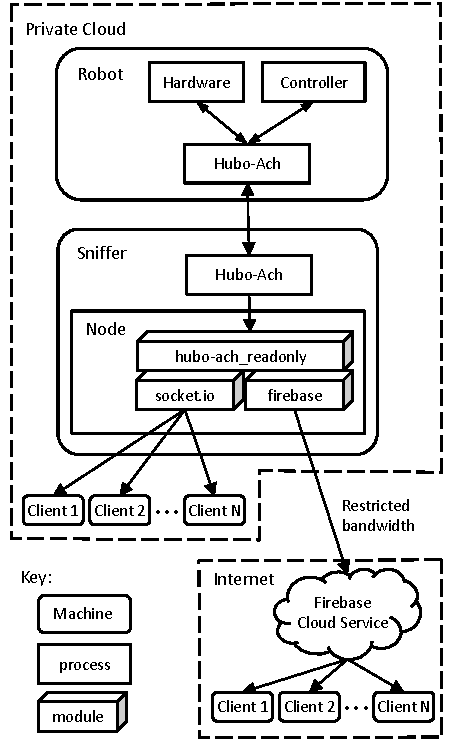
\includegraphics{figures/DetailedOverview.pdf}
  \caption{Detailed overview of system}
  \label{fig:Overview}
\end{figure}

Fig. \ref{fig:Overview} shows a general overview of the system.
% Transition to CAN-bus etc is too jarring.
% Put in a paragraph called "Robot" or something
The Hubo2+ and DRC-Hubo robots operate using a central computer which communicates with the motor control boards and onboard sensors via a CAN bus.
Communicating to the CAN bus is handled by the \texttt{hubo-ach} daemon. \cite{lofaro2013unified}
This communicates with other processes via a shared memory file using the ACH IPC.  \cite{dantam2012robust}
The robot controller and motion planner run as separate processes that communicate with the \texttt{hubo-ach} daemon via the shared memory.
% Don't start the sentence with "because"
% Make sentence positive
% Hubo-ach's remote abilities allow us to offload the webserver 
% hubo-ach remote up to 1kHz over Ethernet
Because the robot computer has limited processing power and its performance is mission critical, we do not to run services such as an HTTP or WebSocket server on the robot itself.
Instead, by using ach network daemon\footnote{\url{http://golems.github.io/ach/manual/\#AEN437}} the shared memory file on the robot is mirrored to another computer on the local network.
This computer acts as the server for our zero-installation robot monitoring webapp.
It runs a ``sniffer'' program that reads robot state data from the shared memory file.

% This should be at the beginning of System Overview.
There are two setup possibilities.
In the most common case, the person monitoring the robot is nearby and connected to the same local wireless network as the robot.
In this scenario, the web application is served up by the computer running the sniffer using a simple HTTP server.
The clients connect by navigating to the IP address of this computer.
Once the interface loads, it connects to the sniffer application via a WebSocket to receive robot state data updates published at a regular frequency.

% Bring up "private cloud" vs "public cloud" options
% Explain how the bandwidth between the robot and the cloud is fixed, and does not depend on the number of users.
% Mention this protects from DNOS attack.
Scenarios might arise however, when the user monitoring the robot is not on the same local network.
For instance, perhaps collaborators from another university want to run the monitoring app, or you want to share the monitoring app with everyone on the Internet so large numbers of people can observe what the robot is doing.
% Delete this. Replace with "situational awareness".
(Such a scenario might make sense at large robotics competitions, for instance, to generate publicity for one's team.)
For this use case, we developed a ``cloud'' approach.
Instead of hosting a web server on the local robot network, the application is hosted by a hosting provider.
% Bring up scaling earlier in Methodology.
To make scaling easy, our web application requires no server-side logic.
A static file hosting provider like Github Pages\footnote{\url{github.io}} is sufficient.
To distribute robot state updates, we use a third-party cloud service called Firebase.\footnote{\url{https://www.firebase.com/}}
The sniffer program only maintains one connection, to Firebase's servers, where it streams robot state data.
The Firebase servers then connect to every browser running the interface and forward incoming data from the sniffer in near real-time (latency on the order of less than half a second).
This allows potentially hundreds or thousands of users to monitor the robot, while having lower network stress than the locally hosted scenario.

\subsection{Server Implementation}
\todo[inline]{Revised}
The primary of the system design was to be highly portable and zero installation.
Because the client interface is web-based, the only part of the system that has to be installed is the server.
Traditional HTTP servers such as Apache can be complicated to install and configure, particularly if the server-side logic requires installing additional environments such as PHP.
For our implementation, we used a platform called \textit{Node}\footnote{\url{http://nodejs.org/}} as the backend.

Node is a platform built on top of the V8 JavaScript engine used in Google Chrome.
It includes an HTTP server in its core modules, and many user-written modules are available.
All modules are installed by the built-in package manager that comes with Node, called \texttt{npm}.
This makes it very easy to specify the dependencies of a piece of software and install them, regardless of what OS you run Node on.

The authors support open source software development.
Thus all of the source code for our interface is available at: \url{https://bitbucket.org/wmhilton/drchubo.js}
The server software was tested on Ubuntu 12.04 LTS because that is what our lab uses to operate our Hubo robots.
However, the client side of course is cross-platform and supported by multiple browsers and operating systems.

The server publishes robot states at a periodic interval.
After optimizing the performance as described in the next section, we were able to achieve updates at 30 frames per second (FPS).
An update rate of 30 FPS resulted in very smooth animations in the interface that were pleasing to the eye.
However, for practical purposes the framerate was reduced to 10 FPS because a human's reaction time is no better than 1/10th of a second, so faster frame rates (while aesthetically pleasing) were not of much practical value for monitoring the robot. \cite{kosinski2008literature}
This cut down on bandwidth.

The advantage of using a cloud service like Firebase is that the burden of scaling a webserver to support large loads is not on the developer.\todo[inline]{Cover in more detail!!!}

\subsection{Client Interface}
\todo[inline]{TODO: Rework}
We chose to write the client in HTML5 + JavaScript in order to be cross-platform, zero-install, and future-proof.
The goal of our interfaces was to improve situational awareness of the robot operator, who may or may not be within a line of sight of the robot.

There are two interfaces we developed.
The first is a graphical qualitative interface, that shows the pose, orientation, and force-torque data of the robot as a 3D model that can be rotated, panned, and zoomed. \ref{fig:Qualitative}.
The second is a quantitative interface, which shows the joint reference positions, encoder values, sensor data, and motor board error flags in a table. \ref{fig:Quantitative}.
These two representations complement each other: the qualitative interface shows the big picture, and the quantitative interface provides the fine details.
Screenshots of the interfaces are shown in Fig. \ref{fig:Screenshots}.

% Remove (limited bandwidth) bit. Make the connection between the robot and the Internet what is "limited bandwidth"
\begin{figure*}[ptb]
    \centering
    \begin{subfigure}[b]{2.5in}
        \centering
        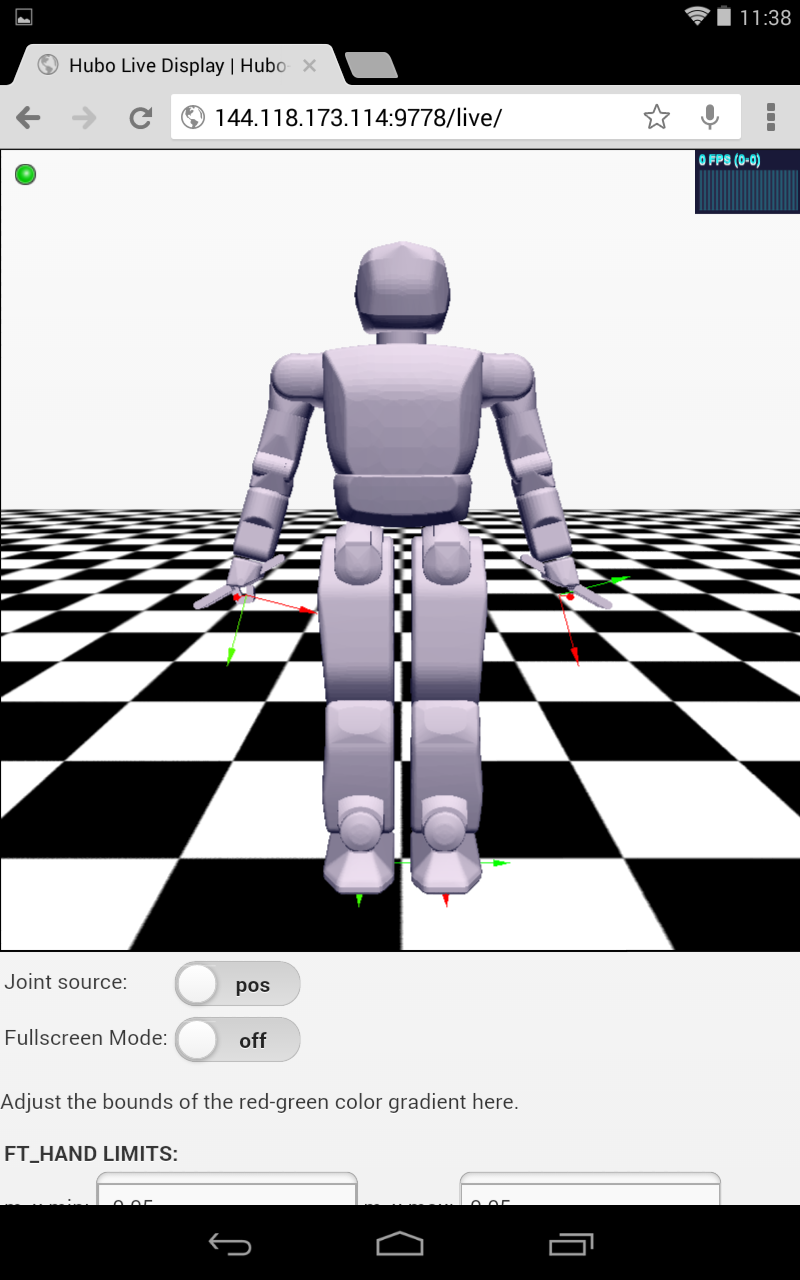
\includegraphics[width=2in]{figures/QualitativePortrait.png}
        \caption{The qualitative interface displays the robot's pose, as well as force-torque information.}
        \label{fig:Qualitative}
    \end{subfigure}%
    \quad
    \begin{subfigure}[b]{2.5in}
        \centering
        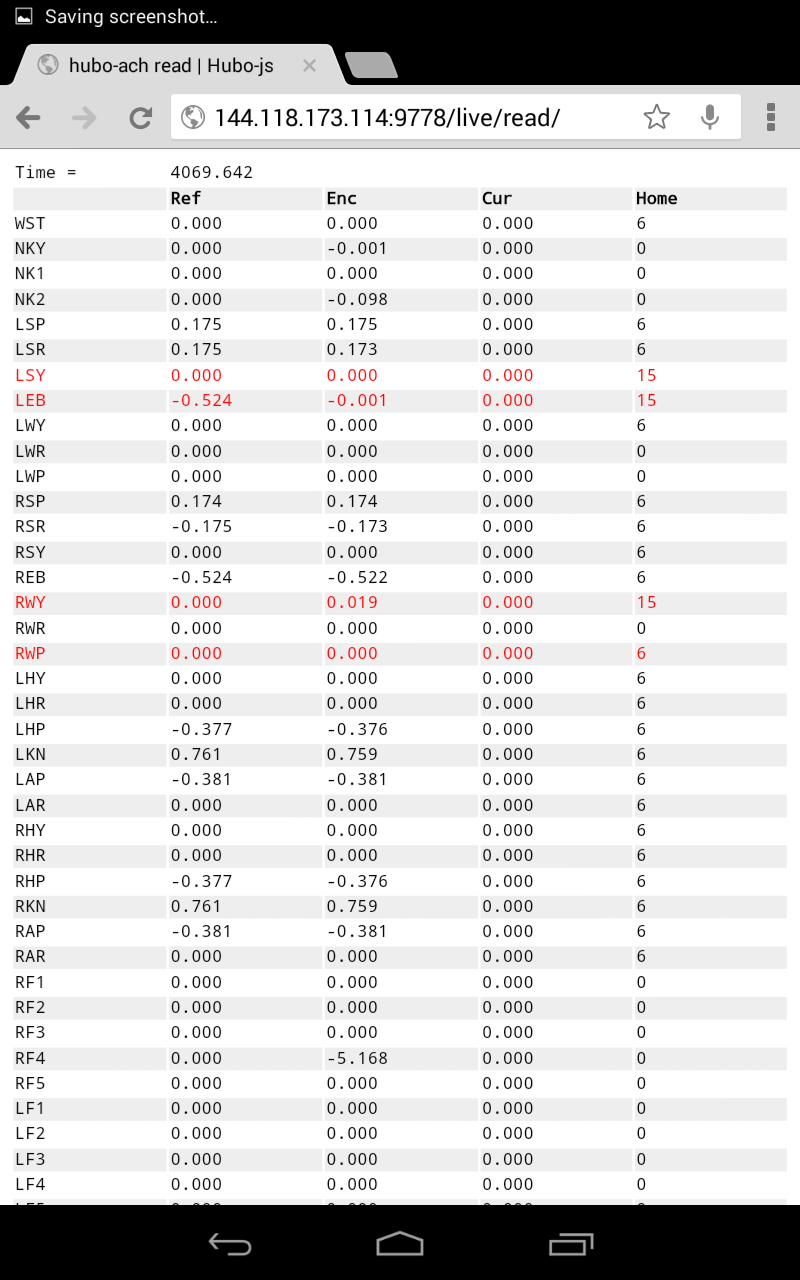
\includegraphics[width=2in]{figures/QuantitativePortrait.png}
        \caption{The quantitative interface displays detailed information about each joint. }
        \label{fig:Quantitative}
    \end{subfigure}%
    \caption{Screenshots of the interfaces}
    \todo[inline]{Final figures?}
    \label{fig:Screenshots}
\end{figure*}

Two interfaces were provided to handle two different modes of analysis.
The first interface is a visual, qualitative display.
The robot's state is represented with the pose, orientation, and color of the 3D model.
The second interface is a numerical, quantitative display.
The robot's state values are displayed directly in a tabular format.
The first interface is useful for getting an overall sense of the robot's performance and making sure it is behaving correctly.
The second interface is useful for debugging and includes the status of individual motor boards.
When it becomes apparent that a joint is not moving or a force torque sensor is miscalibrated, examining the numerical display provides more exacting insight.
The qualitative visual interface is described in this section.

The 3D models used by this visualization tool come from the open source Hubo-in-the-Browser project, which is an ongoing project to make a virtual Hubo that can be programmed and simulated in the browser.\footnote{\url{wmhilton.github.io/hubo-js}}
The models themselves are the same URDF models used in the OpenHubo robot simulator that is based on OpenRAVE. \cite{zhang2013motion}
To import the model into JavaScript, Hubo-in-the-Browser parses the URDF file for the model and loads the individual body meshes using the \textit{Three.js} library.\footnote{\url{threejs.org}}
Both meshes in Collada or STL format are supported.
From the kinematic information in the URDF file, a hierarchical virtual robot object is constructed in JavaScript.
Within this virtual robot object is an array of joint objects.
Changing the value property of the joint object triggers a function that changes the 3D model by rotating the appropriate links and re-renders it.
However, because rendering operations are computationally expensive, in practice we disable autorendering and only re-render the robot after all of its joint values have been updated.
% State in introduction that it was tested on these two platforms.
Because the kinematic models for the robot are not hard-coded by loaded dynamically, it was straightforward for us to develop the same app for both Hubo 2+ and DRC-Hubo.

% Turn off motor controllers to pose in a waving position. Move all limbs some.
% Remove (limited bandwidth) bit. Make the connection between the robot and the Internet what is "limited bandwidth"
\begin{figure*}[ptb]
    \centering
    \begin{subfigure}[b]{3in}
        \centering
        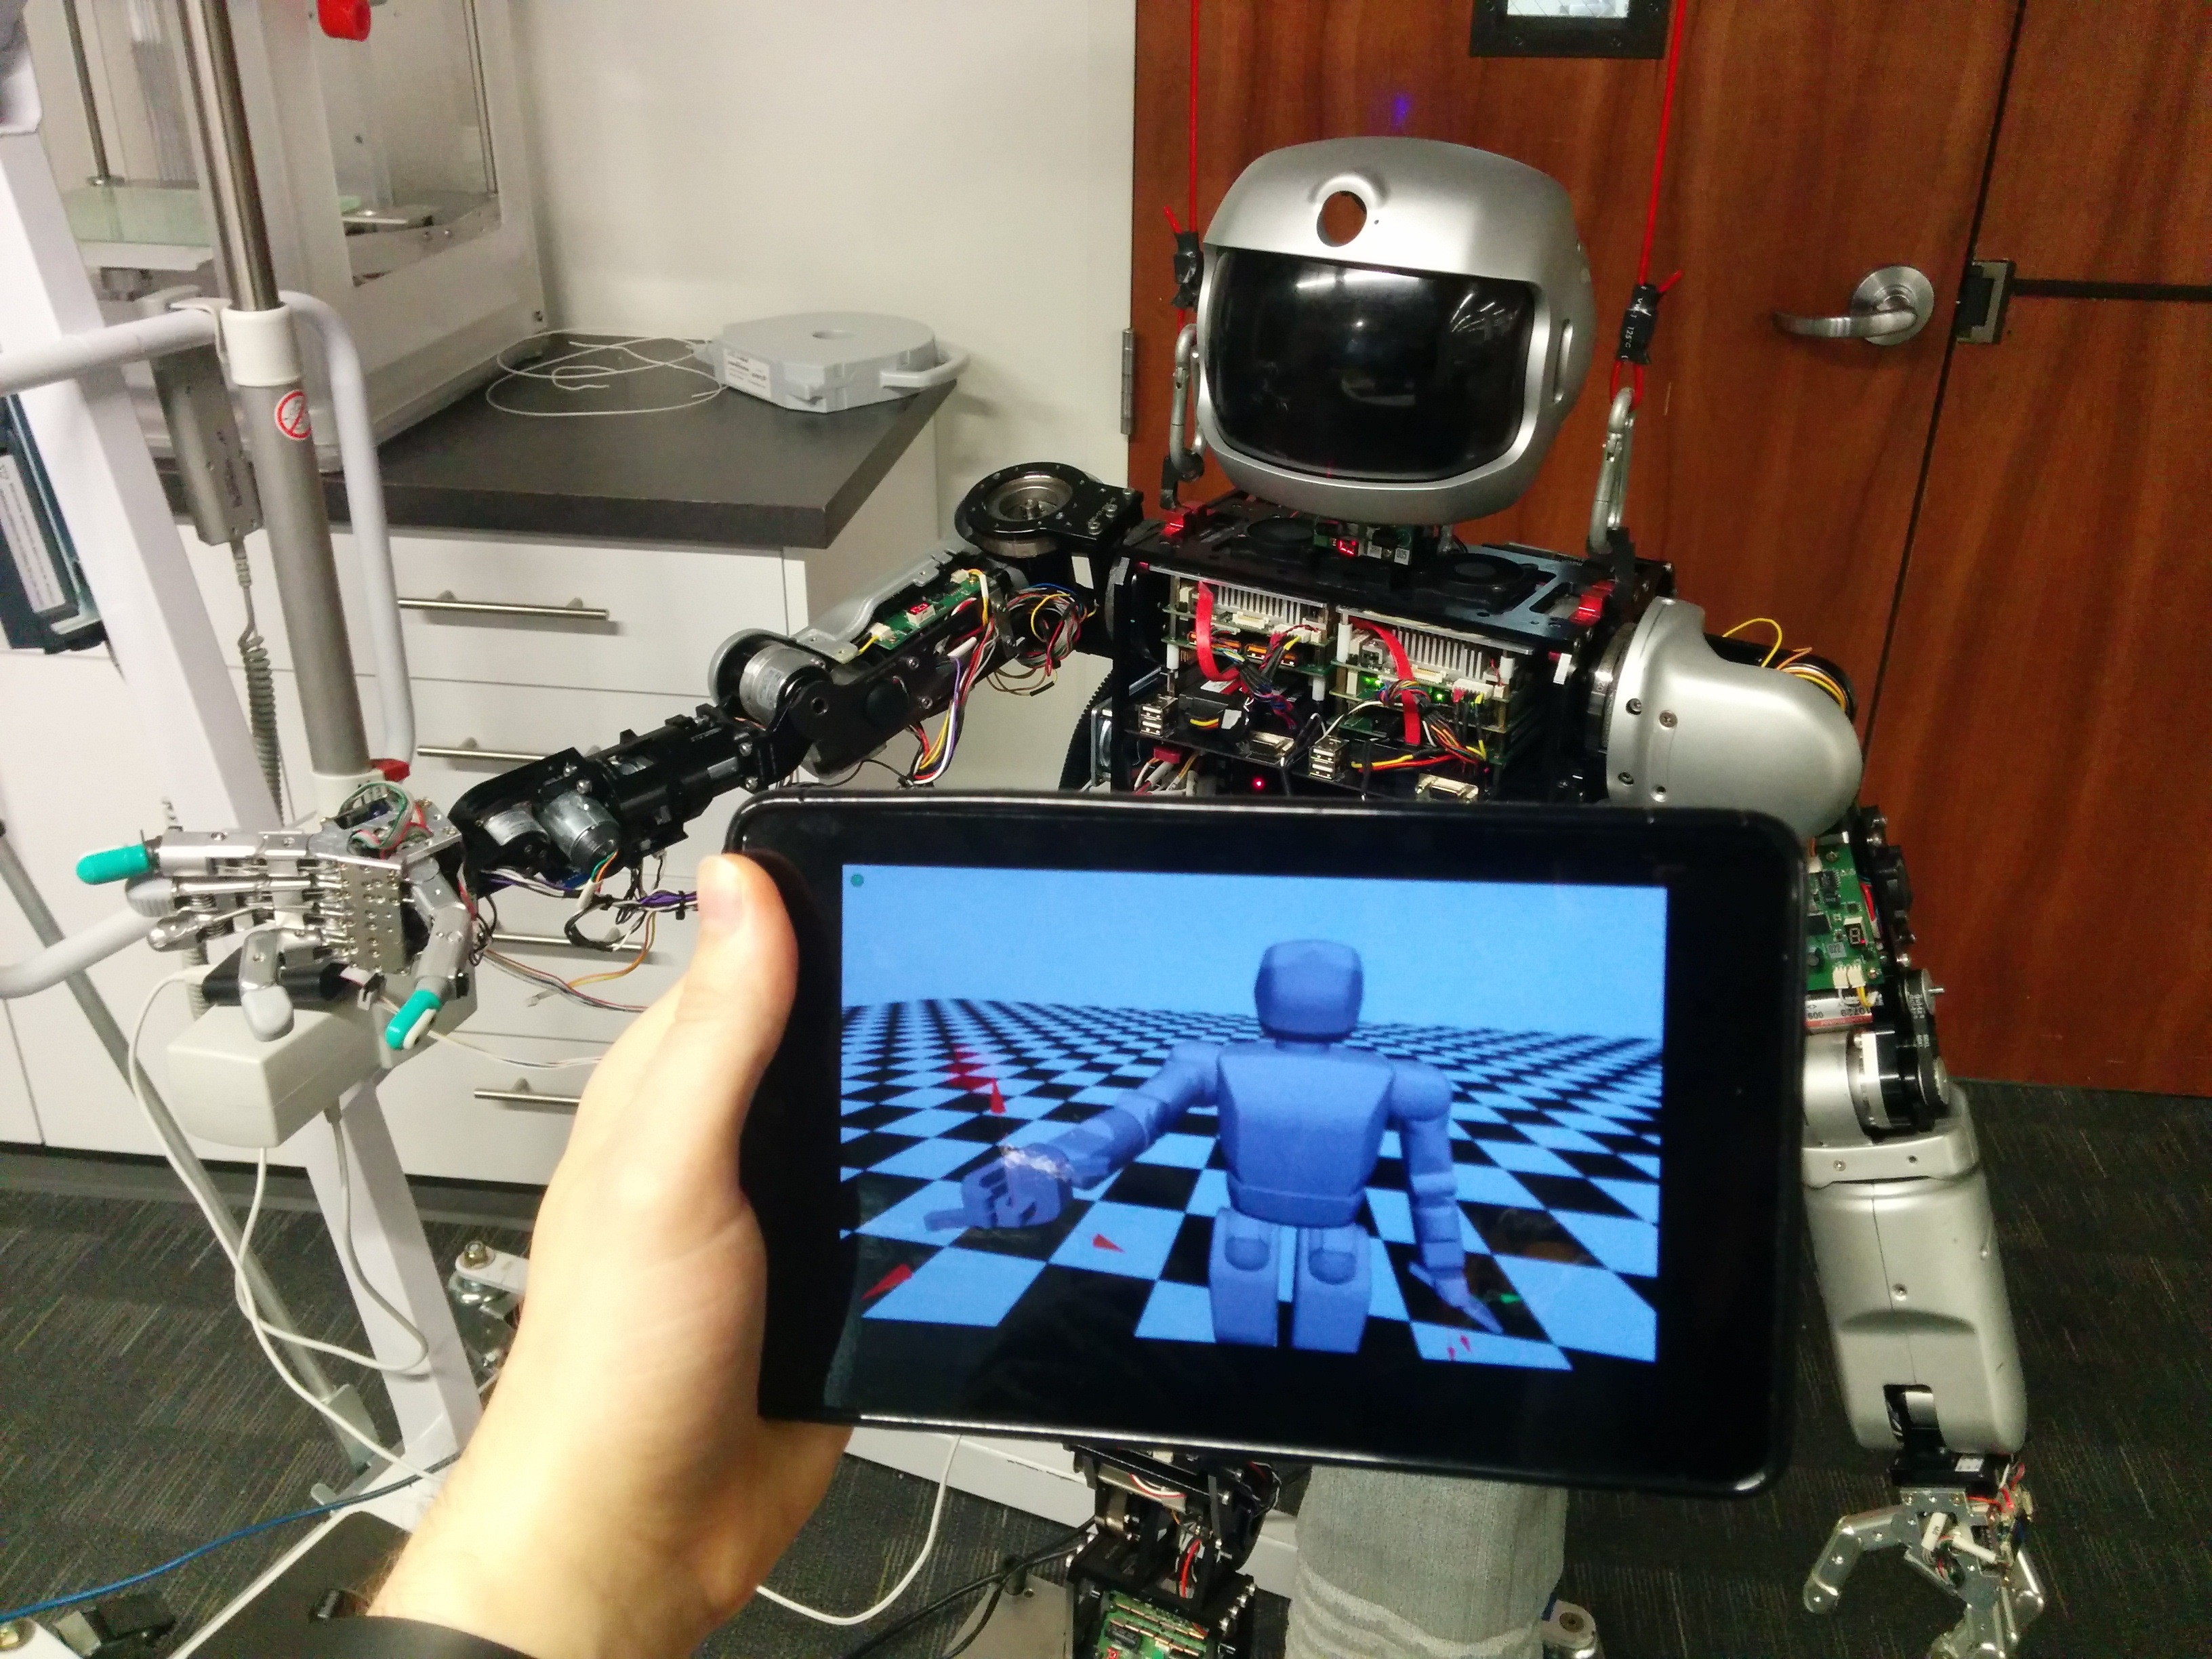
\includegraphics[width=3in]{figures/hubo.jpg}
        \caption{Demo on a Nexus 7 tablet in front of Hubo 2+.}
        \label{fig:Hubo}
    \end{subfigure}%
    \quad
    \begin{subfigure}[b]{3in}
        \centering
        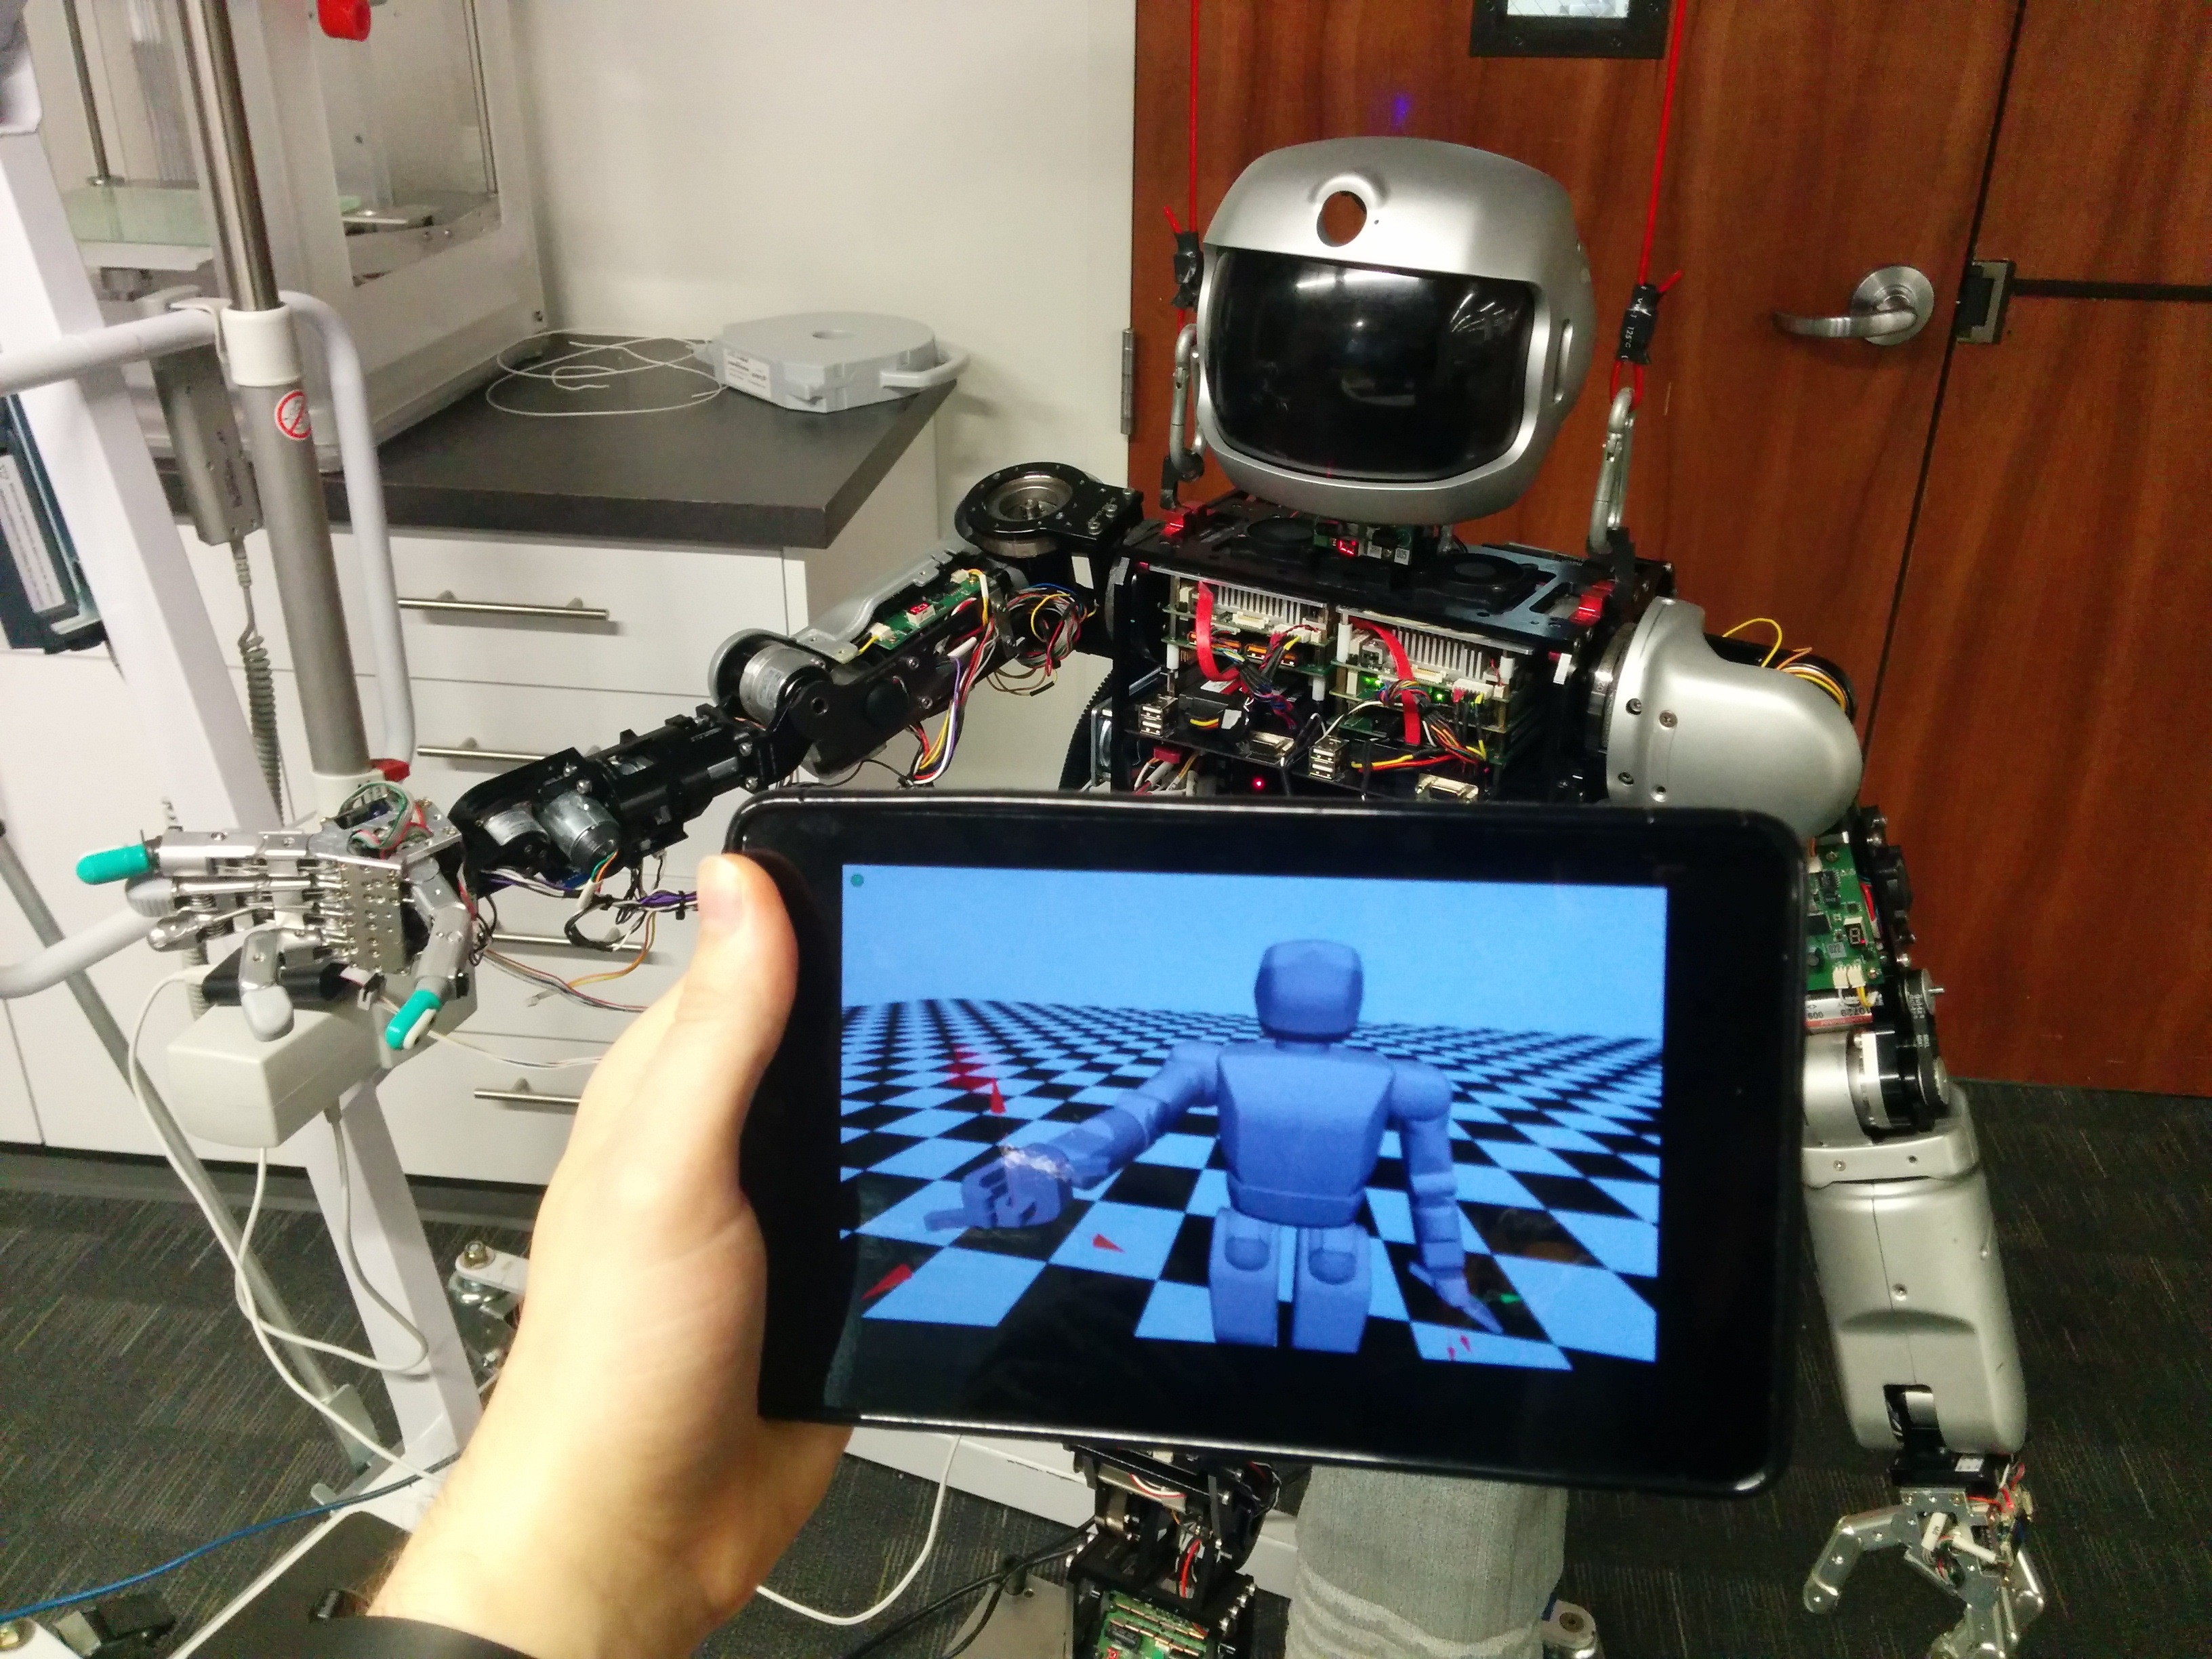
\includegraphics[width=3in]{figures/hubo.jpg}
        \caption{Demo on a Nexus 5 phone in front of DRC Hubo.}
        \label{fig:DRCHubo}
    \end{subfigure}%
    \caption{Photos of the qualitative display in full screen mode in front of the robot(s).}
    \todo[inline]{God I still need better figures.}
    \label{fig:Photos}
\end{figure*}

The following robot state information is displayed by the client:

\subsubsection{Joint Positions}
\todo[inline]{TODO: Rework}
% Goals: is the robot over-torquing itself
% Is it in desired pose 
% This allows the user to easily see this and use their smarts
The interface visualized joint angles by setting joint angles on the WebGL robot model.
Two sets of angles are displayable:
\begin{itemize}
\item The ``pos'' or position angles are the angles reported by the joint encoders.
\item The ``ref'' or reference angles are the commanded angles, the set point for the controllers. 
\end{itemize}
Toggling between the two views immediately reveals any large discrepancy between the desired joint angles and the actual angles.
Discrepancies tend to happen when there is a motor malfunction causing a motor to stop moving, or if a collision with an object is causing the limb to be unable to reach its target pose.

Another situation where discrepancies occur is when certain joints were set to be in a compliant mode.
During walking, for instance, DRC Hubo would enable compliance in the shoulder joints allowing the arms to swing side to side.
This could be observed in the ``pos'' mode, but not in the ``ref'' mode since the arms were not being commanded to swing.
One alternative to having a toggle switch was considered: showing both sets of angles at once using two robot models, where the reference angle model is made partially transparent.
This is the approach used in OpenHubo. 
However, this would have doubled the amount of geometry being rendered by the application, and transparency is more computationally expensive.
In order to ensure the interface was fast and responsive, we opted for this toggle switch approach instead.

\todo{Insert a paragraph explaining the quantitative interface. Joints with errors light up red, etc.}

\subsubsection{Force Torque Sensors}
\todo[inline]{TODO: Rework}
Both Hubo 2+ and DRC Hubo have force-torque sensors in the wrists and ankles that measure the normal force, and the two moments perpendicular to the normal force.
(That is, it does not measure the moment around the normal.)
These measurements were visualized as vectors emanating from the hands and feet of the robot, seen in Fig. \ref{fig:Qualitative}).
A major goal working with humanoid robots in the field is keeping the robot safe.
Therefore the primary goal of the force-torque visuals was to alert the monitoring user if too much force was being exerted on the ankles and wrists.
Users wanted to know when the robot was lifting something that was heavy enough to risk breaking the wrist, or was exerting more than the usual amount of force on its ankles.
Too much force for an extended period of time could cause the ankle motors to burn out.
Therefore the force-torque vectors' colors are mapped to green, yellow, or red. 
Green means the force is within a safe range, red means a risky range, and yellow means in between.
The exact values to use as thresholds between green, yellow, and red can be set by the user in the web interface.

\subsubsection{Inertial Measurement Unit}
\todo[inline]{TODO: Rework}
Both Hubo 2+ and DRC Hubo have an inertial motion unit (IMU) in the torso and one in each leg.
Only the torso IMU was visualized in the qualitative interface; however, up to 3 IMUs were displayed in the quantitative interface.
The primary use of the torso IMU was to indicate the orientation of the robot against the ground.
Of all the data to be monitored, this is one of the most important, particularly for tasks like ladder climbing and walking.
A poor orientation could indicate the robot was not well placed or did not have a good grip on the ladder.
At any time, orientation gives a good indication of whether the robot is tipping or has fallen.
% Through experience, it is beneficial to increase the users situational awareness if there is no line-of-sight.
Because the monitoring user could rotate the 3D graphical model of the robot in all three axis, the orientation of the robot on the screen was not sufficient indication of the robot's orientation in real life.
To properly visualize the orientation of the robot, a reference plane was inserted in the visualization at the robot's foot level.
% Make "better situational awareness" a key focus issue of the paper. One of the goals mentioned originally.

\subsection{Optimizations}
\todo[inline]{Revised}
While the primary components of the system (Three.js, Node, and Firebase / Socket.IO) are all relatively easy to use, optimizations on the client and server were needed to achieve the high throughput and smooth rendering performance of our system.
The initial prototype of the system relied naively on the Firebase API.
On the server side, it would upload a JSON structure of the robot state every update.
On the client side, event handlers were triggered for every updated joint.
This was a simple and intuitive scheme.
However, the initial prototype of the system did not perform well, and experienced severe lag (up to several seconds) and could cause the browser to hang.
This was largely due to the fact that dozens of asynchronous events were being triggered for what was really just one state update.
In later versions of the system, instead of using one message per joint / sensor, all the data was serialized into JSON format and sent as a single string.
Thus on the client end, only a single function was run once per update.
The event handler would deserialize the data, update the joint rotations of the 3D model, and then render the model.

Because Firebases have a fixed amount of bandwidth per month (5GB for the free developer plan), to further reduce bandwidth, the server only sends out messages if the state of the robot changes.
In fact, we round all the state values to 3 decimal places during the serialization to eliminate state changes caused by encoder noise.
The server only transmits the serialized data if the message string is different from the previous message string.
When the private cloud option was developed using Socket.IO, this helped free up local bandwidth for other devices.

%%%%%%%%%%%%%%%%%%%%%%%%%%%%%%%%%%%%%%%%%%%%%%%%%%%%%%%%%%%%%%%%%%%%%%%%%%%%%%%%
\section{RESULTS}
\todo[inline]{New}
The interface was tested on a variety of platforms to verify its cross-platform compatibility.
These tests were done using the private cloud interface (i.e. the socket.io backend, not the Firebase backend).
For mobile testing, we used a Nexus 5 smartphone and the Nexus 7 tablet by Google.
For desktop testing, we used the author's laptop, which happens to be a Toshiba Portege z835 ultrabook.
Testing for OSX and iOS were done on Apple hardware for obvious reasons.
The results of desktop testing are shown in Table \ref{tab:DesktopTesting}.
The results of mobile testing are shown in Table \ref{tab:MobileTesting}.

\begin{table}[h]
\begin{center}
\begin{threeparttable}[b]
\caption{Desktop Testing}
\label{tab:DesktopTesting}
\begin{tabular}{|c|c|c|c|c|c|}
\hline         & \multicolumn{4}{|c|}{Windows 7 (Toshiba Portege z835)} & \multicolumn{1}{|c|}{OSX} \\ 
\hline          & IE 11            & Chrome 32 & Firefox 26       & Opera 19 & Safari 7 \\ 
\hline Hubo 2+  & \xmark \tnote{1} & \cmark    & \cmark \tnote{2} & \cmark   & \cmark  \tnote{2} \tnote{,3} \\ 
\hline DRC Hubo & \cmark \tnote{2} & \cmark    & \cmark \tnote{2} & \cmark   & \cmark  \tnote{2} \tnote{,3} \\ 
\hline 
\end{tabular} 
\begin{tablenotes}
\item [1] Hubo 2+ doesn't work in IE because the COLLADA file loader is broken in IE. DRC Hubo uses STL files so it works.
\item [2] Fullscreen mode doesn't work.
\item [3] WebGL has to be enabled in the ``Develop'' menu.
\end{tablenotes}
\end{threeparttable}
\end{center}
\end{table}
\begin{table}[h]
\begin{center}
\begin{threeparttable}[b]
\caption{Mobile Testing}
\label{tab:MobileTesting}
\begin{tabular}{|c|c|c|c|c|c|c|}
\hline         & \multicolumn{4}{|c|}{Android 4.4 (Nexus 5)} & \multicolumn{2}{|c|}{iPad 3000} \\ 
\hline         & Chrome & Firefox          & Dolphin          & Opera  & Chrome & Safari \\ 
\hline Hubo 2+ & \cmark & \cmark \tnote{1} & \xmark \tnote{2} & \cmark &        & \\ 
\hline DRC Hubo& \cmark & \cmark \tnote{1} & \xmark \tnote{2} & \cmark &        & \\ 
\hline 
\end{tabular} 
\begin{tablenotes}
\item [1] There is noticeable lag in the touch interface however.
\item [2] Lack of WebGL results in unresponsiveness.
\end{tablenotes}
\end{threeparttable}
\end{center}
\end{table}

%%%%%%%%%%%%%%%%%%%%%%%%%%%%%%%%%%%%%%%%%%%%%%%%%%%%%%%%%%%%%%%%%%%%%%%%%%%%%%%%
\section{CONCLUSIONS}
\todo[inline]{New}
% Cross-platform
% Increases situational awareness
We have developed a cross-platform system for monitoring humanoid robots to improve the situational awareness of the robot operators.
% Zero install
%   for these platforms
By creating a web interface, we have eliminated the need for users to install any special software.
% Mobile
%   tested on phone and tablet
The system works well on both desktop and mobile devices, and has been tested on laptops, the Nexus 5 smart phone, and the Nexus 7 tablet.
% Runs on cloud services (public/private)
%   tested on both
The system has been tested in both private and public cloud configuration.
% Tested on two platforms
The interface has been tested on two hardware platforms, the Hubo 2+ and DRC Hubo.

%%%%%%%%%%%%%%%%%%%%%%%%%%%%%%%%%%%%%%%%%%%%%%%%%%%%%%%%%%%%%%%%%%%%%%%%%%%%%%%%
\section{FUTURE WORK}
\todo[inline]{Revised}
One of the advantages of using the \textit{Three.js} library for rendering is that there is a software rendering fallback if WebGL is not supported in the browser.
In the future, we could adapt to the users' browser by detecting if WebGL is unavailable, and downloading a special ``low polygon count'' version of the robot that will render efficiently on browsers using software rendering.
This will increase the number of devices supported.

The system described in this paper only addresses feedback from the robot.
We are currently working on adding feedforward ability, so that users can control the robot from the interface.
Future work will involve how to deal with multiple users all connected to the robot and trying to control it at the same time.
Negotiating which client has control of the robot, or deciding how multiple users can do simultaneous control, are ongoing research.

Lastly, we hope to make the system useful to a wider audience by integrating it with more types of robots.
The 3D interface already works with ROS's URDF format so many types of robots could be loaded into the interface.
Since the underlying Websocket technology is similar to that used by the Rosbridge suite, we are looking at adapting the interface to work with the Rosbridge suite.


%%%%%%%%%%%%%%%%%%%%%%%%%%%%%%%%%%%%%%%%%%%%%%%%%%%%%%%%%%%%%%%%%%%%%%%%%%%%%%%%
\bibliographystyle{ieee/IEEEtran}
\bibliography{ieee/IEEEabrv,references}
\end{document}
